\documentclass[tikz,border=8pt]{standalone}
\usepackage{helvet}
\renewcommand{\familydefault}{\sfdefault}
\usetikzlibrary{decorations.pathmorphing}
\begin{document}
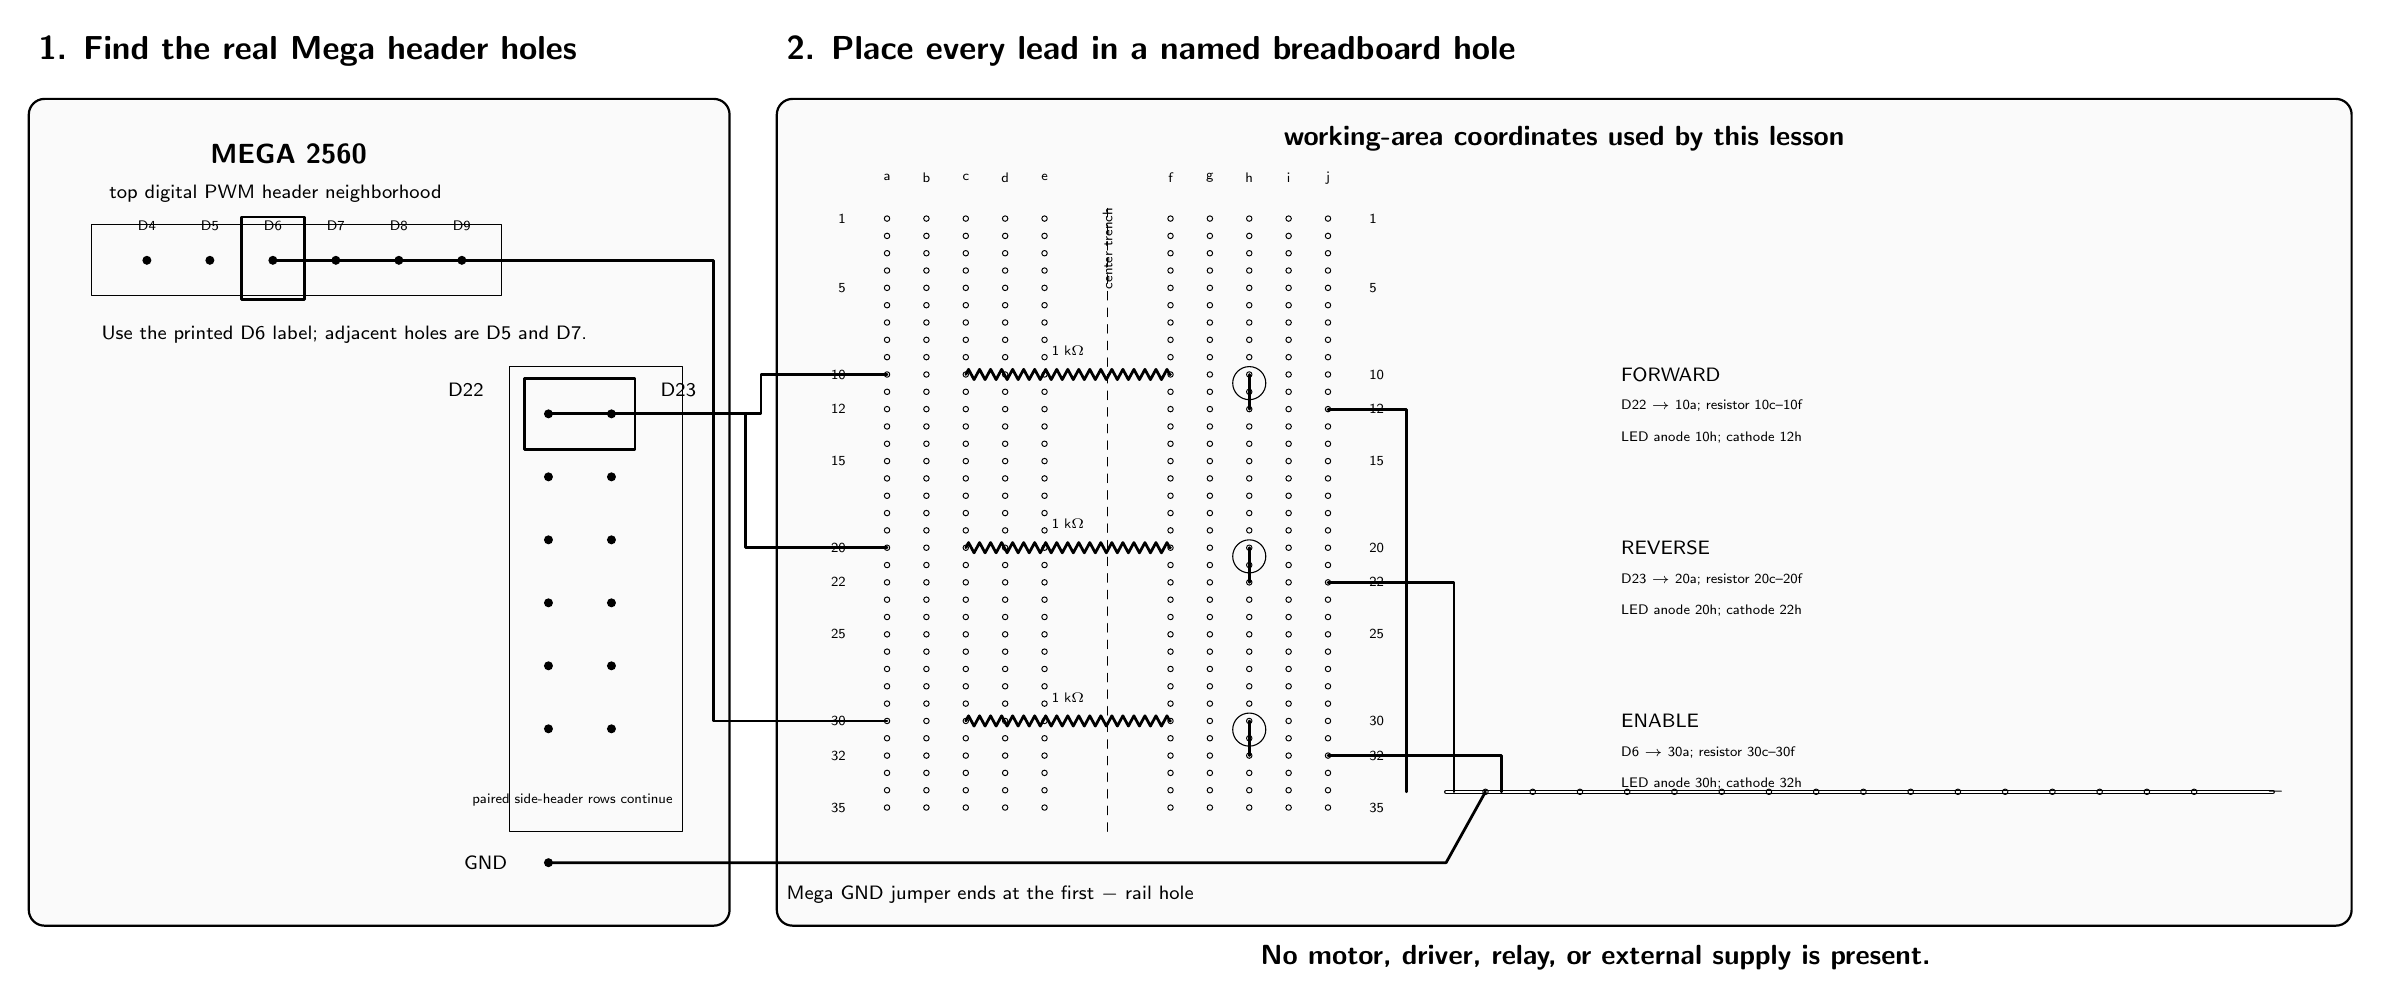
\begin{tikzpicture}[x=1mm,y=1mm,line cap=round,line join=round,
  board/.style={draw,line width=.8pt,rounded corners=2mm,fill=black!2},
  hole/.style={circle,draw,line width=.35pt,inner sep=.7pt},
  pin/.style={circle,fill=black,inner sep=1.15pt},
  wire/.style={line width=1pt},
  tiny/.style={font=\fontsize{5.5}{6}\selectfont},
  small/.style={font=\scriptsize}]

\node[anchor=west,font=\bfseries\large] at (3,119) {1. Find the real Mega header holes};
\node[anchor=west,font=\bfseries\large] at (98,119) {2. Place every lead in a named breadboard hole};

% Mega locator with two physically distinct header regions.
\draw[board] (3,8) rectangle (92,113);
\node[font=\bfseries] at (36,106) {MEGA 2560};
\draw (11,88) rectangle (63,97);
\node[small,anchor=west] at (12,101) {top digital PWM header neighborhood};
\foreach \p/\x in {4/18,5/26,6/34,7/42,8/50,9/58}
{
  \node[pin] at (\x,92.5) {};
  \node[tiny,anchor=south] at (\x,95) {D\p};
}
\draw[line width=1pt] (30,87.5) rectangle (38,98);
\node[small,anchor=west] at (11,83) {Use the printed D6 label; adjacent holes are D5 and D7.};

\draw (64,20) rectangle (86,79);
\foreach \r in {0,...,5}
{
  \pgfmathsetmacro{\yy}{73-\r*8}
  \node[pin] at (69,\yy) {};
  \node[pin] at (77,\yy) {};
}
\draw[line width=1pt] (66,68.5) rectangle (80,77.5);
\node[small,anchor=east] at (62,76) {D22};
\node[small,anchor=west] at (82,76) {D23};
\node[tiny,anchor=east] at (86,24) {paired side-header rows continue};
\node[pin] at (69,16) {};
\node[small,anchor=east] at (65,16) {GND};

% Full physical breadboard.
\draw[board] (98,8) rectangle (298,113);
\node[small,font=\bfseries] at (198,108) {working-area coordinates used by this lesson};

% Column labels and selected numbered rows.
\foreach \c/\x in {a/112,b/117,c/122,d/127,e/132,f/148,g/153,h/158,i/163,j/168}
  \node[tiny] at (\x,103) {\c};
\node[tiny,rotate=90,fill=black!2] at (140,94) {center trench};
\draw[dashed,line width=.5pt] (140,20) -- (140,100);

% Rows 1..35, physical five-hole groups.
\foreach \r in {1,...,35}
{
  \pgfmathsetmacro{\yy}{100-\r*2.2}
  \foreach \x in {112,117,122,127,132,148,153,158,163,168}
    \node[hole] at (\x,\yy) {};
}
\foreach \r in {1,5,10,12,15,20,22,25,30,32,35}
{
  \pgfmathsetmacro{\yy}{100-\r*2.2}
  \node[tiny,anchor=east] at (108,\yy) {\r};
  \node[tiny,anchor=west] at (172,\yy) {\r};
}

% Negative rail with literal holes.
\draw[double,line width=.45pt] (183,25) -- (288,25);
\node[small,anchor=west] at (286,25) {$-$};
\foreach \x in {188,194,...,278}
  \node[hole] at (\x,25) {};

% Row 10: D22 -> 10a, resistor 10c--10f, LED 10h(anode)--12h(cathode), ground.
\pgfmathsetmacro{\rten}{100-10*2.2}
\pgfmathsetmacro{\rtwelve}{100-12*2.2}
\draw[wire] (69,73) -- (96,73) -- (96,\rten) -- (112,\rten);
\draw[wire,decorate,decoration={zigzag,segment length=1.4mm,amplitude=.65mm}]
  (122,\rten) -- (148,\rten);
\node[tiny] at (135,\rten+3) {1 k$\Omega$};
\draw[wire] (158,\rten) -- (158,\rtwelve);
\draw (158,\rten-1.1) circle (2.1);
\draw[wire] (168,\rtwelve) -- (178,\rtwelve) -- (178,25);
\node[small,anchor=west] at (204,\rten) {FORWARD};
\node[tiny,anchor=west] at (204,\rten-4) {D22 $\rightarrow$ 10a; resistor 10c--10f};
\node[tiny,anchor=west] at (204,\rten-8) {LED anode 10h; cathode 12h};

% Row 20: D23 path.
\pgfmathsetmacro{\rtwenty}{100-20*2.2}
\pgfmathsetmacro{\rtwentytwo}{100-22*2.2}
\draw[wire] (77,73) -- (94,73) -- (94,\rtwenty) -- (112,\rtwenty);
\draw[wire,decorate,decoration={zigzag,segment length=1.4mm,amplitude=.65mm}]
  (122,\rtwenty) -- (148,\rtwenty);
\node[tiny] at (135,\rtwenty+3) {1 k$\Omega$};
\draw[wire] (158,\rtwenty) -- (158,\rtwentytwo);
\draw (158,\rtwenty-1.1) circle (2.1);
\draw[wire] (168,\rtwentytwo) -- (184,\rtwentytwo) -- (184,25);
\node[small,anchor=west] at (204,\rtwenty) {REVERSE};
\node[tiny,anchor=west] at (204,\rtwenty-4) {D23 $\rightarrow$ 20a; resistor 20c--20f};
\node[tiny,anchor=west] at (204,\rtwenty-8) {LED anode 20h; cathode 22h};

% Row 30: D6 path.
\pgfmathsetmacro{\rthirty}{100-30*2.2}
\pgfmathsetmacro{\rthirtytwo}{100-32*2.2}
\draw[wire] (34,92.5) -- (90,92.5) -- (90,\rthirty) -- (112,\rthirty);
\draw[wire,decorate,decoration={zigzag,segment length=1.4mm,amplitude=.65mm}]
  (122,\rthirty) -- (148,\rthirty);
\node[tiny] at (135,\rthirty+3) {1 k$\Omega$};
\draw[wire] (158,\rthirty) -- (158,\rthirtytwo);
\draw (158,\rthirty-1.1) circle (2.1);
\draw[wire] (168,\rthirtytwo) -- (190,\rthirtytwo) -- (190,25);
\node[small,anchor=west] at (204,\rthirty) {ENABLE};
\node[tiny,anchor=west] at (204,\rthirty-4) {D6 $\rightarrow$ 30a; resistor 30c--30f};
\node[tiny,anchor=west] at (204,\rthirty-8) {LED anode 30h; cathode 32h};

% Ground rail jumper.
\draw[wire] (69,16) -- (183,16) -- (188,25);
\node[small,anchor=west] at (98,12) {Mega GND jumper ends at the first $-$ rail hole};

\node[font=\bfseries] at (202,4)
  {No motor, driver, relay, or external supply is present.};
\end{tikzpicture}
\end{document}
